\chapter{Registerallocatie}
Graph coloring om registers te alloceren in een interference graph.


Met sommige knopen geen rekening houden (bv h, want er zullen toch twee kleuren overblijven want heeft maar 2 buren).

\begin{enumerate}
	\item Vereenvoudig de graaf door continue knopen met een graad $< k$ weg te laten. Steek ze op een stack.
	\item Pop and color: selecteer een kleur en voeg knoop terug toe met die kleur aan de graaf.
\end{enumerate} 

\section{Register Coalescing}
Knopen die kopieën bevatten proberen samen te voegen als die het kleuren hoogstwaarschijnlijk niet bemoeilijken.

Twee heuristieken die het kleuren zeker niet moeilijker maken:
\begin{itemize}
	\item heuristiek van Briggs: als samengevoegde knoop minder dan $K$ buren van significante graad heeft
	\item heuristiek van George: Elke buur $t$ van $a$ is ofwel een buur van $b$ ofwel niet van significante graad.
\end{itemize}

Figuur \ref{fig:graph_coalescing} illustreert het algoritme en bestaat uit een aantal operaties.

\begin{figure}
	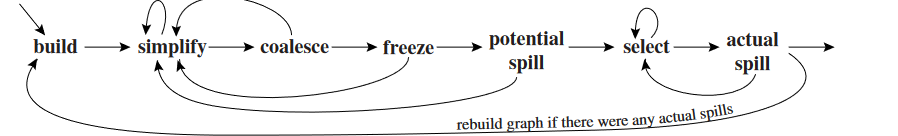
\includegraphics[width=\textwidth]{graph_coalescing}
	\caption{Graafkleuring met \textit{coalescing}.}
	\label{fig:graph_coalescing}
\end{figure}

\begin{itemize}
	\item \textbf{Build:} Construeer de interferentiegraaf en markeer elke knoop als \textit{move-related} of \textit{non-move-related}. Een \textit{move-related} knoop is een knoop dat ofwel het doel of de bron is van een \textit{move} instructie.
	\item \textbf{Simplify:} Verwijder iteratief één \textit{non-move-related} knoop die  graad minder dan $K$ heeft.
	\item \textbf{Coalesce:} Pas \textit{conservative coalescing} toe op de gereduceerde graaf met behulp van Briggs of George. \textbf{Simplify} en \textbf{Coalesce} wordt uitgevoerd tot dat er 
	\item \textbf{Freeze:} Als zowel \textit{simplify} als \textit{coalesce} niet toepasbaar zijn, wordt er een \textit{move-related} knoop bevrozen. Dit heeft als gevolg dat elke \textit{move-related} verbinding naar die knoop geschrapt wordt. Nu wordt \textbf{Simplify} en \textbf{Coalesce} uitgevoerd.
	\item \textbf{Potential Spill:} Als er geen knopen zijn met een graad kleiner dan $K$, een knoop wordt geselecteerd en wordt een \textit{potential spill}.
	\item \textbf{Select:} Pop de hele stack en ken kleuren toe aan de knopen.
	\item \textbf{Actual spill:} Als er een knoop niet gekleurd kan worden, wordt het een echte \textit{spill}. Het programma moet herschreven worden, maar door de variabele in het geheugen op te slaan. De graaf wordt ook opnieuw opgebouwd (figuur \ref{fig:example_spilling}).
	\begin{figure}[ht]
		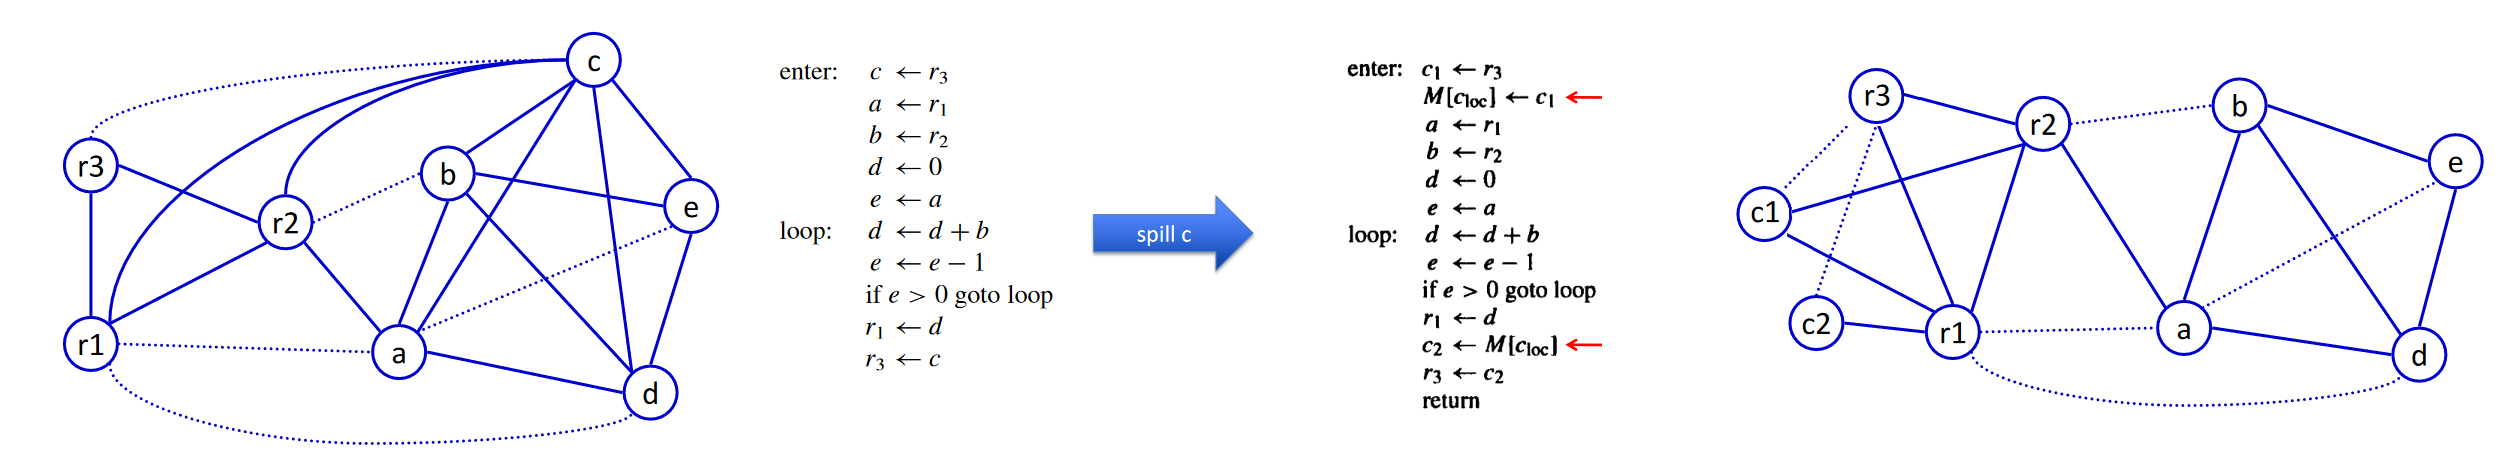
\includegraphics[width=\textwidth]{example_spilling}
		\caption{De knoop $c$ was eerst een potentiële spill, maar kon niet meer gekleurd worden. Het programma moet herschreven worden zodat er twee nieuwe temporaries $c_1$ en $c_2$ ontstaan, die elk een kortere liveness range hebben dan de originele $c$ waardoor er minder interferentie is met andere temporaries.}
		\label{fig:example_spilling}
	\end{figure}

\end{itemize}